% Compile with selfArx.cls in the same folder.
\documentclass[10pt]{selfArx}

\usepackage[english]{babel}
\usepackage{booktabs,tabularx,array}
\usepackage{colortbl}
\usepackage{enumitem}
\usepackage{setspace}
\usepackage{hyperref}
\usepackage{tikz}
\usetikzlibrary{arrows.meta,positioning,shapes.geometric}

\renewcommand{\rmdefault}{ptm}
\setstretch{0.98}
\setlength{\columnsep}{0.52cm}
\setlength{\floatsep}{4pt}
\setlength{\textfloatsep}{5pt}
\setlength{\intextsep}{4pt}
\setlist[itemize]{leftmargin=12pt,itemsep=0pt,topsep=2pt}
\setlist[enumerate]{leftmargin=14pt,itemsep=0pt,topsep=2pt}
\definecolor{color1}{RGB}{0,0,0}
\definecolor{color2}{RGB}{0,102,204}
\definecolor{blockD}{RGB}{224,242,254}
\definecolor{blockF}{RGB}{254,242,214}
\definecolor{blockP}{RGB}{236,236,236}
\hypersetup{hidelinks,colorlinks=true,urlcolor=color2,citecolor=color1,linkcolor=color1,
  pdftitle={Generic Warehouse Simulation Framework},pdfauthor={IE305 Group}}

\newcolumntype{L}{>{\raggedright\arraybackslash}X}
\newcolumntype{P}[1]{>{\raggedright\arraybackslash}p{#1}}

\JournalInfo{IE305 Simulation Lab, IEOR@IITB}
\Archive{Simulation Project}
\Keywords{}
\PaperTitle{A Generic Simulation Framework for Warehouse Handling Systems with Automatic Model Generation}
\Authors{Shivam Soni (24B4525) Siddhesh Phadke (24B4502)}

\raggedbottom
\begin{document}

\Abstract{Warehouses decide where to put storage and pickup areas, how many docks and forklifts to run and which operating rules to follow, usually by rules of thumb. Each new layout normally needs a new simulation model, which is slow and requires an expert. We want to build one generic, parameter driven discrete event model of a warehouse, covering inbound receiving, putaway, order picking, staging and outbound shipping, that a non-expert can configure and run. On top of this framework we plan to develop an automatic model generation framework: the user draws a facility on a grid of standard building blocks and the complete simulation model is generated from it. The framework is used to size the forklift fleet, compare storage and pickup allotments and test policies under synthetic stochastic demand.}
\maketitle
\thispagestyle{empty}

% =====================================================
\section{System Selection \& Problem Statement}

\subsection*{The System}
A warehouse handling system: trucks arrive and wait in a yard, unload at a dock, pallets are checked and put away to storage, customer orders trigger picking, picked pallets are staged in pickup areas and loaded onto outbound trucks. The model is built in three components:
\begin{itemize}
  \item \textbf{User Interface:} a non-expert sets layout, docks, forklifts, volume and policies, launches experiments and reads a KPI dashboard.
  \item \textbf{Generic Modelling Framework:} reusable building blocks (Dock, Forklift/charging, Passage), generic process logic and generic agents for trucks, pallets, orders and forklifts.
  \item \textbf{Data \& Model Assembly:} stores configurations and input distributions, assembles the runnable model and exports results.
\end{itemize}
\begin{figure}[h]
    \centering
    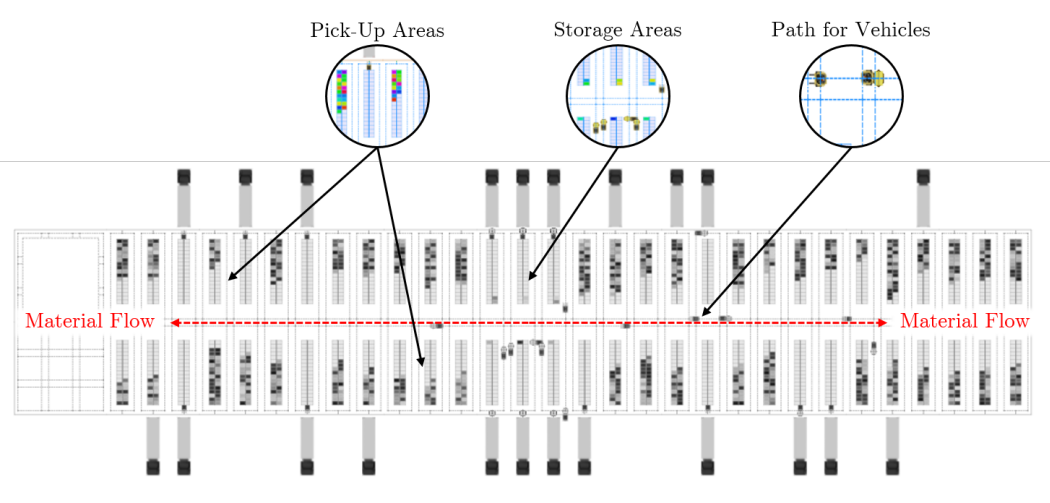
\includegraphics[width=1\linewidth]{idea_warehouse.png}
    \caption{Simulation Model}
    \label{fig:placeholder}
\end{figure}
\subsection*{Highlight: Automatic Model Generation}
\noindent{\color{color2}\vrule width 2pt}\hspace{0pt}\colorbox{color2!10}{\parbox{\dimexpr\columnwidth-2\fboxsep-2pt\relax}{\small Building a new AnyLogic model for every layout is the main cost of simulation-based layout planning. We want to generate it automatically. The user fills a grid matrix where each cell is a building block (D = dock block, F = forklift block, P = passage, 0 = empty). A generator reads the matrix and creates the space markup, walls, docks, storage and pickup areas and the forklift path network at runtime. Any facility shape (I, L, T, U, H) then becomes a one-click experiment instead of a modelling task. This is built as an extension on top of the working framework.}}

\begin{figure}[H]
\centering
\resizebox{\columnwidth}{!}{%
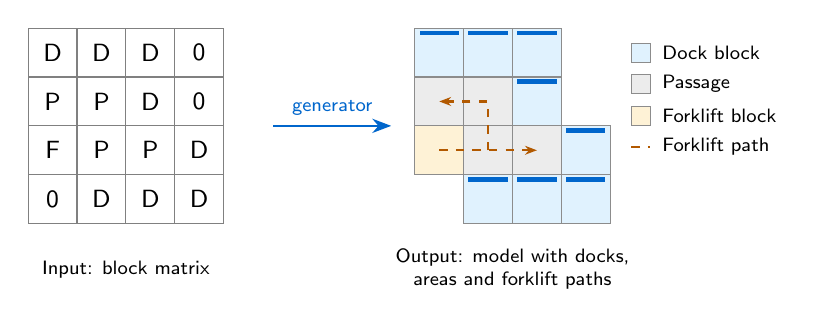
\begin{tikzpicture}[font=\sffamily\small,
  cell/.style={draw=black!50, minimum size=0.62cm, inner sep=0pt},
  arr/.style={-{Stealth[length=2.4mm]}, thick, color=color2}]
% Matrix input (L-shape)
\foreach \r/\row in {0/{D,D,D,0},1/{P,P,D,0},2/{F,P,P,D},3/{0,D,D,D}}{
  \foreach \c [count=\i from 0] in \row {
    \node[cell] at (\i*0.62, -\r*0.62) {\c};
  }
}
\node[font=\sffamily\scriptsize, align=center] at (0.93,-2.75) {Input: block matrix};
% Arrow
\draw[arr] (2.8,-0.93) -- node[above, font=\sffamily\scriptsize]{generator} (4.3,-0.93);
% Generated layout
\foreach \x/\y/\t in {0/0/D,1/0/D,2/0/D,2/1/D,3/2/D,1/3/D,2/3/D,3/3/D}{
  \filldraw[fill=blockD, draw=black!45] (4.6+\x*0.62, -\y*0.62-0.31) rectangle ++(0.62,0.62);
  \fill[color2] (4.6+\x*0.62+0.06, -\y*0.62+0.22) rectangle ++(0.5,0.06);
}
\foreach \x/\y in {0/1,1/1,1/2,2/2}{
  \filldraw[fill=blockP, draw=black!45] (4.6+\x*0.62, -\y*0.62-0.31) rectangle ++(0.62,0.62);
}
\filldraw[fill=blockF, draw=black!45] (4.6, -2*0.62-0.31) rectangle ++(0.62,0.62);
\draw[orange!70!black, thick, dashed, -{Stealth[length=1.5mm]}] (4.91,-1.24) -- (6.15,-1.24);
\draw[orange!70!black, thick, dashed, -{Stealth[length=1.5mm]}] (5.53,-1.24) -- (5.53,-0.62) -- (4.91,-0.62);
% Legend
\foreach \c/\l/\yy in {blockD/Dock block/0, blockP/Passage/-0.4, blockF/Forklift block/-0.8}{
  \filldraw[fill=\c, draw=black!45] (7.35,\yy-0.12) rectangle ++(0.24,0.24);
  \node[anchor=west, font=\sffamily\scriptsize] at (7.62,\yy) {\l};
}
\draw[orange!70!black, thick, dashed] (7.35,-1.2) -- ++(0.24,0);
\node[anchor=west, font=\sffamily\scriptsize] at (7.62,-1.2) {Forklift path};
\node[font=\sffamily\scriptsize, align=center] at (5.84,-2.75) {Output: model with docks,\\areas and forklift paths};
\end{tikzpicture}}
\caption{Automatic model generation: a block matrix is converted into a complete, runnable facility model.}
\end{figure}

\subsection*{The Problem}
Poorly allotted storage and pickup areas and poorly routed material flow cause excess forklift travel, dock congestion and late truck departures. We study:
\begin{enumerate}
  \item \textbf{Allotment \& flow:} how should storage areas, pickup areas, vehicle paths and yard capacity be allotted to minimise travel and cycle time?
  \item \textbf{Resources:} what minimum forklift fleet and dock count meets the service level at peak, and which resource is the bottleneck?
  \item \textbf{Policies:} how much do dock, storage and dispatching rules improve performance at zero capital cost?
  \item \textbf{Usability:} can one generic model, and ultimately one generated from a drawing, answer these without manual rebuilding?
\end{enumerate}
% \newpage
\subsection*{System Boundaries}
{\footnotesize
\renewcommand{\arraystretch}{1.05}
\setlength{\tabcolsep}{3pt}
\noindent\begin{tabularx}{\columnwidth}{LL}
\rowcolor{color2!14} \textbf{Included} & \textbf{Excluded} \\
Truck arrival, yard queue, docking & Gate check-in, yard manoeuvring \\
Unloading, receiving check, putaway & External road transport \\
Order arrival, picking, staging, loading & Replenishment, SKU slotting \\
Forklift travel, congestion, charging & Shifts and breaks \\
Dock, storage, dispatch policies & Returns, damages, IT \\
\end{tabularx}}



% =====================================================
\section{System Configuration}

\subsection*{Entities \& Resources}
{\small
\renewcommand{\arraystretch}{1.15}
\setlength{\tabcolsep}{3pt}
\noindent\begin{tabularx}{\columnwidth}{>{\bfseries}P{2.3cm}L}
\rowcolor{color2!14} Entity & Attributes \\
Inbound truck  & Arrival time, pallets, assigned dock \\
Outbound truck & Departure time, destination \\
Pallet         & SKU class, storage location \\
Customer order & Lines per order, due time \\
\rowcolor{color2!14} Resource & Capacity / decision \\
Dock doors       & Count; inbound share \\
Forklifts        & Fleet size \\
Storage area     & Slots; placement \\
Pickup / staging & Capacity; placement \\
Yard             & Truck waiting slots \\
Chargers         & Count \\
\end{tabularx}}

\subsection*{Process Flow Sketch}
\begin{figure}[H]
\centering
\resizebox{\columnwidth}{!}{%
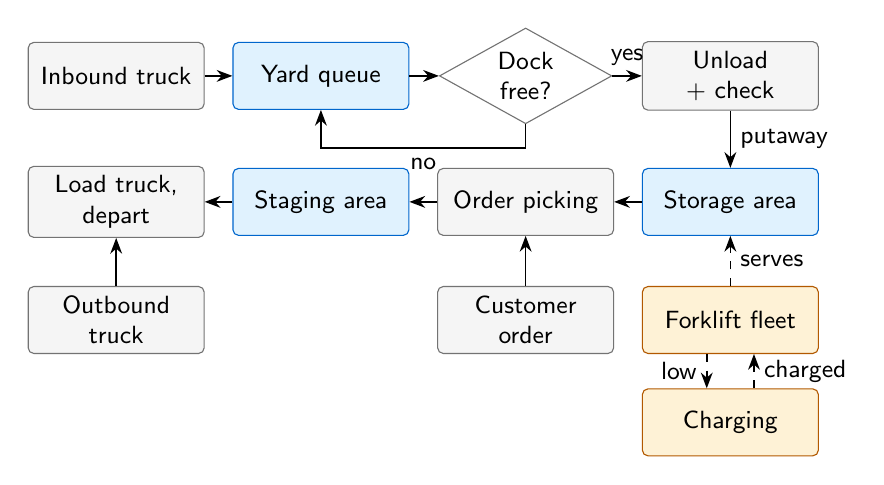
\begin{tikzpicture}[font=\sffamily\small,
  box/.style={draw=black!55, rounded corners=2pt, align=center, minimum height=0.85cm, text width=2.0cm, fill=blockP!50},
  res/.style={draw=color2, rounded corners=2pt, align=center, minimum height=0.85cm, text width=2.0cm, fill=blockD},
  dec/.style={draw=black!55, diamond, aspect=1.8, inner sep=0.5pt, text width=1.0cm, align=center, fill=white},
  arr/.style={-{Stealth[length=2mm]}, semithick}]
\node[box] (a1) at (0,0)     {Inbound truck};
\node[res] (y)  at (2.6,0)   {Yard queue};
\node[dec] (d)  at (5.2,0)   {Dock free?};
\node[box] (u)  at (7.8,0)   {Unload + check};
\node[box] (l)  at (0,-1.6)   {Load truck, depart};
\node[res] (st) at (2.6,-1.6) {Staging area};
\node[box] (pk) at (5.2,-1.6) {Order picking};
\node[res] (s)  at (7.8,-1.6) {Storage area};
\node[box] (a2) at (0,-3.1)   {Outbound truck};
\node[box] (o)  at (5.2,-3.1) {Customer order};
\node[res,fill=blockF,draw=orange!70!black] (f) at (7.8,-3.1) {Forklift fleet};
\node[res,fill=blockF,draw=orange!70!black] (c) at (7.8,-4.4) {Charging};
\draw[arr] (a1)--(y); \draw[arr] (y)--(d);
\draw[arr] (d)--node[above]{yes}(u);
\draw[arr] (d.south)--++(0,-0.3)-|node[pos=0.25,below]{no}(y.south);
\draw[arr] (u)--node[right]{putaway}(s);
\draw[arr] (s)--(pk); \draw[arr] (pk)--(st); \draw[arr] (st)--(l);
\draw[arr] (a2)--(l); \draw[arr] (o)--(pk);
\draw[arr,dashed] (f)--node[right]{serves}(s);
\draw[arr,dashed] ([xshift=-3mm]f.south)--node[left]{low}([xshift=-3mm]c.north);
\draw[arr,dashed] ([xshift=3mm]c.north)--node[right]{charged}([xshift=3mm]f.south);
\end{tikzpicture}}
\caption{Routing logic. Blue: queues and areas with finite capacity; orange: forklift resource loop.}
\end{figure}

% =====================================================
\section{Input Data Collection Plan}
All inputs use synthetic data. Distributions are fitted in Python, checked with KS / Chi-square tests, and the model is run on both sampled data and fitted distributions.

{\small
\renewcommand{\arraystretch}{1.12}
\setlength{\tabcolsep}{3pt}
\noindent\begin{tabularx}{\columnwidth}{LP{1.35cm}P{2.6cm}}
\rowcolor{color2!14} \textbf{Stochastic variable} & \textbf{Sourcing} & \textbf{Sample / Dist.} \\
Inbound truck inter-arrival & Synthetic & 500; Exponential \\
Outbound departure time     & Synthetic & 200; Uniform \\
Pallets per truck           & Synthetic & 500; Empirical \\
Order inter-arrival         & Synthetic & 1000; Exponential \\
Lines per order             & Synthetic & 1000; Geometric \\
Unload / load time          & Synthetic & 500; Lognormal \\
Pick time per line          & Synthetic & 500; Lognormal \\
Forklift speed              & Synthetic & Normal \\
Charge time                 & Synthetic & Uniform \\
Forklift MTBF / MTTR        & Synthetic & 200; Exp. / Lognormal \\
SKU class mix               & Synthetic & Uniform vs.\ skewed \\
\end{tabularx}}

% =====================================================
% \newpage
\section{Output Measures \& Optimization Goal}

\subsection*{Key Performance Indicators}
{\small
\renewcommand{\arraystretch}{1.12}
\setlength{\tabcolsep}{3pt}
\noindent\begin{tabularx}{\columnwidth}{>{\bfseries}P{1.8cm}L}
\rowcolor{color2!14} Category & KPI \\
Time        & Cycle time, truck turnaround (mean, p95), yard wait \\
Throughput  & Pallets, orders, trucks per shift \\
Utilisation & Forklifts, docks, storage, staging (\%) \\
Distance    & Total forklift travel distance \\
Congestion  & Yard queue, forklift blocked time, staging overflow \\
\end{tabularx}}

\subsection*{The ``What If'' / Optimization Goal}
{\small
\renewcommand{\arraystretch}{1.12}
\setlength{\tabcolsep}{3pt}
\noindent\begin{tabularx}{\columnwidth}{>{\bfseries}P{2.9cm}L}
\rowcolor{color2!14} Decision variable & Levels \\
Layout form                & I, L, T; any shape via generation \\
Storage / pickup allotment & Near docks, centralised, SKU zones \\
Path direction             & One-way, two-way \\
Docks (inbound share)      & 12, 18, 24 (25, 33, 50\%) \\
Yard capacity              & Low, medium, high \\
Forklift fleet size        & Minimum feasible to saturation \\
Policies                   & Dock, storage, dispatch rules \\
Volume                     & Baseline, +20\%, +40\% \\
\end{tabularx}}

\vspace{4pt}
\noindent\colorbox{color2!10}{\parbox{\dimexpr\columnwidth-2\fboxsep\relax}{\small
\textbf{Optimization goal (OptQuest):} minimise forklift fleet size subject to p95 truck turnaround $\leq T^{*}$ and zero staging overflow; then minimise forklift travel through allotment and policy choice.}}

\begin{thebibliography}{9}\small
\bibitem{wsc} L. Jurgeleit, M. Mowe, M. Kiefer, C. Schumacher, and U. Clausen. Automatic model generation for discrete event simulation of less-than-truckload terminals. \textit{Proc.\ Winter Simulation Conference}, 1493--1504, 2024.
\end{thebibliography}

\end{document}